\documentclass[a4paper, 12pt]{article}
\usepackage{mathtools}
\usepackage{amssymb}
\usepackage[utf8]{inputenc} % special characters

% diagramms
\usepackage{tikz} %diagrams
\usetikzlibrary{arrows,cd,calc} % for commutative diagrams

% template for a simple article in maths, also useful to just type up something math short!

%\newcommand{\invf}{f^{-1}}
%\newcommand{\invg}{g^{-1}}
%opening
\title{}
\author{}
\date{\today}

\begin{document}

\maketitle

\begin{center}
	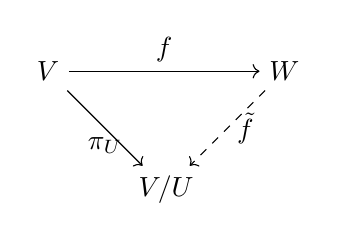
\begin{tikzpicture}
	\node (V) at (0,0) {$V$};
	\node (W) at (3,0) {$W$};
	\node (R) at (1.5,-1.5) {$V\slash U$};
	\draw[->, above] (V) to node {$f$} (W);
	\draw[->, below] (V)  to node {$\pi_U$} (R);
	\draw[->, right, dashed] (W)  to node {$\tilde f$} (R);
	\end{tikzpicture}
\end{center}

\begin{center}
	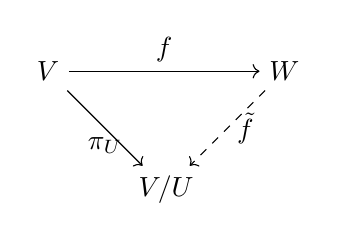
\begin{tikzpicture}
	\node (V) at (0,0) {$V$};
	\node (W) at (3,0) {$W$};
	\node (R) at (1.5,-1.5) {$V\slash U$};
	\draw[->, above] (V) to node {$f$} (W);
	\draw[->, below] (V)  to node {$\pi_U$} (R);
	\draw[->, right, dashed] (W)  to node {$\tilde f$} (R);
	\end{tikzpicture}
\end{center}

\begin{center}
	\begin{tikzcd}
		V \arrow[r, "f"] \arrow[dr, dashrightarrow, "f^{\ast}(\phi)"]
		& W \arrow[d, "\phi"]\\
		& K\\
		V^{\ast} & \arrow[l, "f^{\ast}"] W^{\ast}
	\end{tikzcd}
\end{center}

\begin{center}
	\begin{tikzcd}
		V \arrow[r, "f"] \arrow[d, "\iota_V \cong"] 
			& W \arrow[d, "\iota_W \cong"] \\
		V^{\ast \ast} \arrow[r, "f^{\ast \ast}"] 
		& W^{\ast \ast}
	\end{tikzcd}
\end{center}

\begin{center}
	\begin{tikzpicture}[scale=0.6]
		\draw[thick] (-2,0) -- (10,0) node[right] {$x_1$}; 
		\draw[thick] (0,-2) -- (0,10) node[above] {$x_2$};
		\coordinate (center) at (0,0)
		% triangle
		%\fill[line width=1pt, color=red,fill=red, opacity=0.1] (0,0) -- (2,7) -- (7,2) -- cycle ;
		\draw[red] (2,7) -- (7,2);
		\draw[fill=green] ($(center) + (0:5)$) arc (0:12:5)
		\draw[red] (3.5,3.5) node {\scriptsize $\Delta$};
		%Circles
		\draw[shift={(-7.8,-4.5)}, color=green, opacity=0.1, fill=green] (0,0) -- (0:5.6) arc (0:7.2:5.6) -- cycle
		% Paralello
		\draw[->, thick] (0,0) -- (7,2) node[right] {\scriptsize $x_1=(a,b)$};
		\draw[->, thick] (0,0) -- (2,7) node[above] {\scriptsize$x_2=(c,d)$};
		\draw[->, thick] (7,2) -- (9,9) node[right] {\scriptsize$x_1 + x_2$};
		\draw[->, thick] (2,7) -- (9,9);
		\draw[blue] (0,0) -- (7,2) node[near end, below] {\scriptsize $g_{\Delta}$};
		\draw[blue] (3.5,1) -- (2,7) node[near start, right] {\scriptsize$h_{\Delta}$};
		
	\end{tikzpicture}
\end{center}

\end{document}
